
% Default to the notebook output style

    


% Inherit from the specified cell style.




    
\documentclass[11pt]{article}

    
    
    \usepackage[T1]{fontenc}
    % Nicer default font (+ math font) than Computer Modern for most use cases
    \usepackage{mathpazo}

    % Basic figure setup, for now with no caption control since it's done
    % automatically by Pandoc (which extracts ![](path) syntax from Markdown).
    \usepackage{graphicx}
    % We will generate all images so they have a width \maxwidth. This means
    % that they will get their normal width if they fit onto the page, but
    % are scaled down if they would overflow the margins.
    \makeatletter
    \def\maxwidth{\ifdim\Gin@nat@width>\linewidth\linewidth
    \else\Gin@nat@width\fi}
    \makeatother
    \let\Oldincludegraphics\includegraphics
    % Set max figure width to be 80% of text width, for now hardcoded.
    \renewcommand{\includegraphics}[1]{\Oldincludegraphics[width=.8\maxwidth]{#1}}
    % Ensure that by default, figures have no caption (until we provide a
    % proper Figure object with a Caption API and a way to capture that
    % in the conversion process - todo).
    \usepackage{caption}
    \DeclareCaptionLabelFormat{nolabel}{}
    \captionsetup{labelformat=nolabel}

    \usepackage{adjustbox} % Used to constrain images to a maximum size 
    \usepackage{xcolor} % Allow colors to be defined
    \usepackage{enumerate} % Needed for markdown enumerations to work
    \usepackage{geometry} % Used to adjust the document margins
    \usepackage{amsmath} % Equations
    \usepackage{amssymb} % Equations
    \usepackage{textcomp} % defines textquotesingle
    % Hack from http://tex.stackexchange.com/a/47451/13684:
    \AtBeginDocument{%
        \def\PYZsq{\textquotesingle}% Upright quotes in Pygmentized code
    }
    \usepackage{upquote} % Upright quotes for verbatim code
    \usepackage{eurosym} % defines \euro
    \usepackage[mathletters]{ucs} % Extended unicode (utf-8) support
    \usepackage[utf8x]{inputenc} % Allow utf-8 characters in the tex document
    \usepackage{fancyvrb} % verbatim replacement that allows latex
    \usepackage{grffile} % extends the file name processing of package graphics 
                         % to support a larger range 
    % The hyperref package gives us a pdf with properly built
    % internal navigation ('pdf bookmarks' for the table of contents,
    % internal cross-reference links, web links for URLs, etc.)
    \usepackage{hyperref}
    \usepackage{longtable} % longtable support required by pandoc >1.10
    \usepackage{booktabs}  % table support for pandoc > 1.12.2
    \usepackage[inline]{enumitem} % IRkernel/repr support (it uses the enumerate* environment)
    \usepackage[normalem]{ulem} % ulem is needed to support strikethroughs (\sout)
                                % normalem makes italics be italics, not underlines
    

    
    
    % Colors for the hyperref package
    \definecolor{urlcolor}{rgb}{0,.145,.698}
    \definecolor{linkcolor}{rgb}{.71,0.21,0.01}
    \definecolor{citecolor}{rgb}{.12,.54,.11}

    % ANSI colors
    \definecolor{ansi-black}{HTML}{3E424D}
    \definecolor{ansi-black-intense}{HTML}{282C36}
    \definecolor{ansi-red}{HTML}{E75C58}
    \definecolor{ansi-red-intense}{HTML}{B22B31}
    \definecolor{ansi-green}{HTML}{00A250}
    \definecolor{ansi-green-intense}{HTML}{007427}
    \definecolor{ansi-yellow}{HTML}{DDB62B}
    \definecolor{ansi-yellow-intense}{HTML}{B27D12}
    \definecolor{ansi-blue}{HTML}{208FFB}
    \definecolor{ansi-blue-intense}{HTML}{0065CA}
    \definecolor{ansi-magenta}{HTML}{D160C4}
    \definecolor{ansi-magenta-intense}{HTML}{A03196}
    \definecolor{ansi-cyan}{HTML}{60C6C8}
    \definecolor{ansi-cyan-intense}{HTML}{258F8F}
    \definecolor{ansi-white}{HTML}{C5C1B4}
    \definecolor{ansi-white-intense}{HTML}{A1A6B2}

    % commands and environments needed by pandoc snippets
    % extracted from the output of `pandoc -s`
    \providecommand{\tightlist}{%
      \setlength{\itemsep}{0pt}\setlength{\parskip}{0pt}}
    \DefineVerbatimEnvironment{Highlighting}{Verbatim}{commandchars=\\\{\}}
    % Add ',fontsize=\small' for more characters per line
    \newenvironment{Shaded}{}{}
    \newcommand{\KeywordTok}[1]{\textcolor[rgb]{0.00,0.44,0.13}{\textbf{{#1}}}}
    \newcommand{\DataTypeTok}[1]{\textcolor[rgb]{0.56,0.13,0.00}{{#1}}}
    \newcommand{\DecValTok}[1]{\textcolor[rgb]{0.25,0.63,0.44}{{#1}}}
    \newcommand{\BaseNTok}[1]{\textcolor[rgb]{0.25,0.63,0.44}{{#1}}}
    \newcommand{\FloatTok}[1]{\textcolor[rgb]{0.25,0.63,0.44}{{#1}}}
    \newcommand{\CharTok}[1]{\textcolor[rgb]{0.25,0.44,0.63}{{#1}}}
    \newcommand{\StringTok}[1]{\textcolor[rgb]{0.25,0.44,0.63}{{#1}}}
    \newcommand{\CommentTok}[1]{\textcolor[rgb]{0.38,0.63,0.69}{\textit{{#1}}}}
    \newcommand{\OtherTok}[1]{\textcolor[rgb]{0.00,0.44,0.13}{{#1}}}
    \newcommand{\AlertTok}[1]{\textcolor[rgb]{1.00,0.00,0.00}{\textbf{{#1}}}}
    \newcommand{\FunctionTok}[1]{\textcolor[rgb]{0.02,0.16,0.49}{{#1}}}
    \newcommand{\RegionMarkerTok}[1]{{#1}}
    \newcommand{\ErrorTok}[1]{\textcolor[rgb]{1.00,0.00,0.00}{\textbf{{#1}}}}
    \newcommand{\NormalTok}[1]{{#1}}
    
    % Additional commands for more recent versions of Pandoc
    \newcommand{\ConstantTok}[1]{\textcolor[rgb]{0.53,0.00,0.00}{{#1}}}
    \newcommand{\SpecialCharTok}[1]{\textcolor[rgb]{0.25,0.44,0.63}{{#1}}}
    \newcommand{\VerbatimStringTok}[1]{\textcolor[rgb]{0.25,0.44,0.63}{{#1}}}
    \newcommand{\SpecialStringTok}[1]{\textcolor[rgb]{0.73,0.40,0.53}{{#1}}}
    \newcommand{\ImportTok}[1]{{#1}}
    \newcommand{\DocumentationTok}[1]{\textcolor[rgb]{0.73,0.13,0.13}{\textit{{#1}}}}
    \newcommand{\AnnotationTok}[1]{\textcolor[rgb]{0.38,0.63,0.69}{\textbf{\textit{{#1}}}}}
    \newcommand{\CommentVarTok}[1]{\textcolor[rgb]{0.38,0.63,0.69}{\textbf{\textit{{#1}}}}}
    \newcommand{\VariableTok}[1]{\textcolor[rgb]{0.10,0.09,0.49}{{#1}}}
    \newcommand{\ControlFlowTok}[1]{\textcolor[rgb]{0.00,0.44,0.13}{\textbf{{#1}}}}
    \newcommand{\OperatorTok}[1]{\textcolor[rgb]{0.40,0.40,0.40}{{#1}}}
    \newcommand{\BuiltInTok}[1]{{#1}}
    \newcommand{\ExtensionTok}[1]{{#1}}
    \newcommand{\PreprocessorTok}[1]{\textcolor[rgb]{0.74,0.48,0.00}{{#1}}}
    \newcommand{\AttributeTok}[1]{\textcolor[rgb]{0.49,0.56,0.16}{{#1}}}
    \newcommand{\InformationTok}[1]{\textcolor[rgb]{0.38,0.63,0.69}{\textbf{\textit{{#1}}}}}
    \newcommand{\WarningTok}[1]{\textcolor[rgb]{0.38,0.63,0.69}{\textbf{\textit{{#1}}}}}
    
    
    % Define a nice break command that doesn't care if a line doesn't already
    % exist.
    \def\br{\hspace*{\fill} \\* }
    % Math Jax compatability definitions
    \def\gt{>}
    \def\lt{<}
    % Document parameters
    \title{Z-Transformation}
    
    
    

    % Pygments definitions
    
\makeatletter
\def\PY@reset{\let\PY@it=\relax \let\PY@bf=\relax%
    \let\PY@ul=\relax \let\PY@tc=\relax%
    \let\PY@bc=\relax \let\PY@ff=\relax}
\def\PY@tok#1{\csname PY@tok@#1\endcsname}
\def\PY@toks#1+{\ifx\relax#1\empty\else%
    \PY@tok{#1}\expandafter\PY@toks\fi}
\def\PY@do#1{\PY@bc{\PY@tc{\PY@ul{%
    \PY@it{\PY@bf{\PY@ff{#1}}}}}}}
\def\PY#1#2{\PY@reset\PY@toks#1+\relax+\PY@do{#2}}

\expandafter\def\csname PY@tok@w\endcsname{\def\PY@tc##1{\textcolor[rgb]{0.73,0.73,0.73}{##1}}}
\expandafter\def\csname PY@tok@c\endcsname{\let\PY@it=\textit\def\PY@tc##1{\textcolor[rgb]{0.25,0.50,0.50}{##1}}}
\expandafter\def\csname PY@tok@cp\endcsname{\def\PY@tc##1{\textcolor[rgb]{0.74,0.48,0.00}{##1}}}
\expandafter\def\csname PY@tok@k\endcsname{\let\PY@bf=\textbf\def\PY@tc##1{\textcolor[rgb]{0.00,0.50,0.00}{##1}}}
\expandafter\def\csname PY@tok@kp\endcsname{\def\PY@tc##1{\textcolor[rgb]{0.00,0.50,0.00}{##1}}}
\expandafter\def\csname PY@tok@kt\endcsname{\def\PY@tc##1{\textcolor[rgb]{0.69,0.00,0.25}{##1}}}
\expandafter\def\csname PY@tok@o\endcsname{\def\PY@tc##1{\textcolor[rgb]{0.40,0.40,0.40}{##1}}}
\expandafter\def\csname PY@tok@ow\endcsname{\let\PY@bf=\textbf\def\PY@tc##1{\textcolor[rgb]{0.67,0.13,1.00}{##1}}}
\expandafter\def\csname PY@tok@nb\endcsname{\def\PY@tc##1{\textcolor[rgb]{0.00,0.50,0.00}{##1}}}
\expandafter\def\csname PY@tok@nf\endcsname{\def\PY@tc##1{\textcolor[rgb]{0.00,0.00,1.00}{##1}}}
\expandafter\def\csname PY@tok@nc\endcsname{\let\PY@bf=\textbf\def\PY@tc##1{\textcolor[rgb]{0.00,0.00,1.00}{##1}}}
\expandafter\def\csname PY@tok@nn\endcsname{\let\PY@bf=\textbf\def\PY@tc##1{\textcolor[rgb]{0.00,0.00,1.00}{##1}}}
\expandafter\def\csname PY@tok@ne\endcsname{\let\PY@bf=\textbf\def\PY@tc##1{\textcolor[rgb]{0.82,0.25,0.23}{##1}}}
\expandafter\def\csname PY@tok@nv\endcsname{\def\PY@tc##1{\textcolor[rgb]{0.10,0.09,0.49}{##1}}}
\expandafter\def\csname PY@tok@no\endcsname{\def\PY@tc##1{\textcolor[rgb]{0.53,0.00,0.00}{##1}}}
\expandafter\def\csname PY@tok@nl\endcsname{\def\PY@tc##1{\textcolor[rgb]{0.63,0.63,0.00}{##1}}}
\expandafter\def\csname PY@tok@ni\endcsname{\let\PY@bf=\textbf\def\PY@tc##1{\textcolor[rgb]{0.60,0.60,0.60}{##1}}}
\expandafter\def\csname PY@tok@na\endcsname{\def\PY@tc##1{\textcolor[rgb]{0.49,0.56,0.16}{##1}}}
\expandafter\def\csname PY@tok@nt\endcsname{\let\PY@bf=\textbf\def\PY@tc##1{\textcolor[rgb]{0.00,0.50,0.00}{##1}}}
\expandafter\def\csname PY@tok@nd\endcsname{\def\PY@tc##1{\textcolor[rgb]{0.67,0.13,1.00}{##1}}}
\expandafter\def\csname PY@tok@s\endcsname{\def\PY@tc##1{\textcolor[rgb]{0.73,0.13,0.13}{##1}}}
\expandafter\def\csname PY@tok@sd\endcsname{\let\PY@it=\textit\def\PY@tc##1{\textcolor[rgb]{0.73,0.13,0.13}{##1}}}
\expandafter\def\csname PY@tok@si\endcsname{\let\PY@bf=\textbf\def\PY@tc##1{\textcolor[rgb]{0.73,0.40,0.53}{##1}}}
\expandafter\def\csname PY@tok@se\endcsname{\let\PY@bf=\textbf\def\PY@tc##1{\textcolor[rgb]{0.73,0.40,0.13}{##1}}}
\expandafter\def\csname PY@tok@sr\endcsname{\def\PY@tc##1{\textcolor[rgb]{0.73,0.40,0.53}{##1}}}
\expandafter\def\csname PY@tok@ss\endcsname{\def\PY@tc##1{\textcolor[rgb]{0.10,0.09,0.49}{##1}}}
\expandafter\def\csname PY@tok@sx\endcsname{\def\PY@tc##1{\textcolor[rgb]{0.00,0.50,0.00}{##1}}}
\expandafter\def\csname PY@tok@m\endcsname{\def\PY@tc##1{\textcolor[rgb]{0.40,0.40,0.40}{##1}}}
\expandafter\def\csname PY@tok@gh\endcsname{\let\PY@bf=\textbf\def\PY@tc##1{\textcolor[rgb]{0.00,0.00,0.50}{##1}}}
\expandafter\def\csname PY@tok@gu\endcsname{\let\PY@bf=\textbf\def\PY@tc##1{\textcolor[rgb]{0.50,0.00,0.50}{##1}}}
\expandafter\def\csname PY@tok@gd\endcsname{\def\PY@tc##1{\textcolor[rgb]{0.63,0.00,0.00}{##1}}}
\expandafter\def\csname PY@tok@gi\endcsname{\def\PY@tc##1{\textcolor[rgb]{0.00,0.63,0.00}{##1}}}
\expandafter\def\csname PY@tok@gr\endcsname{\def\PY@tc##1{\textcolor[rgb]{1.00,0.00,0.00}{##1}}}
\expandafter\def\csname PY@tok@ge\endcsname{\let\PY@it=\textit}
\expandafter\def\csname PY@tok@gs\endcsname{\let\PY@bf=\textbf}
\expandafter\def\csname PY@tok@gp\endcsname{\let\PY@bf=\textbf\def\PY@tc##1{\textcolor[rgb]{0.00,0.00,0.50}{##1}}}
\expandafter\def\csname PY@tok@go\endcsname{\def\PY@tc##1{\textcolor[rgb]{0.53,0.53,0.53}{##1}}}
\expandafter\def\csname PY@tok@gt\endcsname{\def\PY@tc##1{\textcolor[rgb]{0.00,0.27,0.87}{##1}}}
\expandafter\def\csname PY@tok@err\endcsname{\def\PY@bc##1{\setlength{\fboxsep}{0pt}\fcolorbox[rgb]{1.00,0.00,0.00}{1,1,1}{\strut ##1}}}
\expandafter\def\csname PY@tok@kc\endcsname{\let\PY@bf=\textbf\def\PY@tc##1{\textcolor[rgb]{0.00,0.50,0.00}{##1}}}
\expandafter\def\csname PY@tok@kd\endcsname{\let\PY@bf=\textbf\def\PY@tc##1{\textcolor[rgb]{0.00,0.50,0.00}{##1}}}
\expandafter\def\csname PY@tok@kn\endcsname{\let\PY@bf=\textbf\def\PY@tc##1{\textcolor[rgb]{0.00,0.50,0.00}{##1}}}
\expandafter\def\csname PY@tok@kr\endcsname{\let\PY@bf=\textbf\def\PY@tc##1{\textcolor[rgb]{0.00,0.50,0.00}{##1}}}
\expandafter\def\csname PY@tok@bp\endcsname{\def\PY@tc##1{\textcolor[rgb]{0.00,0.50,0.00}{##1}}}
\expandafter\def\csname PY@tok@fm\endcsname{\def\PY@tc##1{\textcolor[rgb]{0.00,0.00,1.00}{##1}}}
\expandafter\def\csname PY@tok@vc\endcsname{\def\PY@tc##1{\textcolor[rgb]{0.10,0.09,0.49}{##1}}}
\expandafter\def\csname PY@tok@vg\endcsname{\def\PY@tc##1{\textcolor[rgb]{0.10,0.09,0.49}{##1}}}
\expandafter\def\csname PY@tok@vi\endcsname{\def\PY@tc##1{\textcolor[rgb]{0.10,0.09,0.49}{##1}}}
\expandafter\def\csname PY@tok@vm\endcsname{\def\PY@tc##1{\textcolor[rgb]{0.10,0.09,0.49}{##1}}}
\expandafter\def\csname PY@tok@sa\endcsname{\def\PY@tc##1{\textcolor[rgb]{0.73,0.13,0.13}{##1}}}
\expandafter\def\csname PY@tok@sb\endcsname{\def\PY@tc##1{\textcolor[rgb]{0.73,0.13,0.13}{##1}}}
\expandafter\def\csname PY@tok@sc\endcsname{\def\PY@tc##1{\textcolor[rgb]{0.73,0.13,0.13}{##1}}}
\expandafter\def\csname PY@tok@dl\endcsname{\def\PY@tc##1{\textcolor[rgb]{0.73,0.13,0.13}{##1}}}
\expandafter\def\csname PY@tok@s2\endcsname{\def\PY@tc##1{\textcolor[rgb]{0.73,0.13,0.13}{##1}}}
\expandafter\def\csname PY@tok@sh\endcsname{\def\PY@tc##1{\textcolor[rgb]{0.73,0.13,0.13}{##1}}}
\expandafter\def\csname PY@tok@s1\endcsname{\def\PY@tc##1{\textcolor[rgb]{0.73,0.13,0.13}{##1}}}
\expandafter\def\csname PY@tok@mb\endcsname{\def\PY@tc##1{\textcolor[rgb]{0.40,0.40,0.40}{##1}}}
\expandafter\def\csname PY@tok@mf\endcsname{\def\PY@tc##1{\textcolor[rgb]{0.40,0.40,0.40}{##1}}}
\expandafter\def\csname PY@tok@mh\endcsname{\def\PY@tc##1{\textcolor[rgb]{0.40,0.40,0.40}{##1}}}
\expandafter\def\csname PY@tok@mi\endcsname{\def\PY@tc##1{\textcolor[rgb]{0.40,0.40,0.40}{##1}}}
\expandafter\def\csname PY@tok@il\endcsname{\def\PY@tc##1{\textcolor[rgb]{0.40,0.40,0.40}{##1}}}
\expandafter\def\csname PY@tok@mo\endcsname{\def\PY@tc##1{\textcolor[rgb]{0.40,0.40,0.40}{##1}}}
\expandafter\def\csname PY@tok@ch\endcsname{\let\PY@it=\textit\def\PY@tc##1{\textcolor[rgb]{0.25,0.50,0.50}{##1}}}
\expandafter\def\csname PY@tok@cm\endcsname{\let\PY@it=\textit\def\PY@tc##1{\textcolor[rgb]{0.25,0.50,0.50}{##1}}}
\expandafter\def\csname PY@tok@cpf\endcsname{\let\PY@it=\textit\def\PY@tc##1{\textcolor[rgb]{0.25,0.50,0.50}{##1}}}
\expandafter\def\csname PY@tok@c1\endcsname{\let\PY@it=\textit\def\PY@tc##1{\textcolor[rgb]{0.25,0.50,0.50}{##1}}}
\expandafter\def\csname PY@tok@cs\endcsname{\let\PY@it=\textit\def\PY@tc##1{\textcolor[rgb]{0.25,0.50,0.50}{##1}}}

\def\PYZbs{\char`\\}
\def\PYZus{\char`\_}
\def\PYZob{\char`\{}
\def\PYZcb{\char`\}}
\def\PYZca{\char`\^}
\def\PYZam{\char`\&}
\def\PYZlt{\char`\<}
\def\PYZgt{\char`\>}
\def\PYZsh{\char`\#}
\def\PYZpc{\char`\%}
\def\PYZdl{\char`\$}
\def\PYZhy{\char`\-}
\def\PYZsq{\char`\'}
\def\PYZdq{\char`\"}
\def\PYZti{\char`\~}
% for compatibility with earlier versions
\def\PYZat{@}
\def\PYZlb{[}
\def\PYZrb{]}
\makeatother


    % Exact colors from NB
    \definecolor{incolor}{rgb}{0.0, 0.0, 0.5}
    \definecolor{outcolor}{rgb}{0.545, 0.0, 0.0}



    
    % Prevent overflowing lines due to hard-to-break entities
    \sloppy 
    % Setup hyperref package
    \hypersetup{
      breaklinks=true,  % so long urls are correctly broken across lines
      colorlinks=true,
      urlcolor=urlcolor,
      linkcolor=linkcolor,
      citecolor=citecolor,
      }
    % Slightly bigger margins than the latex defaults
    
    \geometry{verbose,tmargin=1in,bmargin=1in,lmargin=1in,rmargin=1in}
    
    

    \begin{document}
    
    
    \maketitle
    
    

    
    \section{Motivation}\label{motivation}

\begin{itemize}
\item
  Das Ziel der Z-Transformation ist es, ein diskretes zeitabhängiges
  Signal \(x[k]\) in den Bildbereich bzw. Z-Bereich zu Transformieren.
  \(x[k]\) ist hierbei eine Folge aus realen oder komplexen Zahlen
\item
  Diese Transformation in den Z-Bereich wird zum Lösen von linearen
  Differenzengleichungen mit konstanten Koeffizienten verwendet. Diese
  Gleichungen haben die Form
  \(y[k] = b_0 x[k] + \sum_{i=1}^V b_i \cdot x[k-i] - \sum_{i=1}^U a_i \cdot y[k-i]\)
\item
  Die Differenzengleichungen im Zeitbereich werden im Bildbereich zu
  algebraischen Gleichungen. Damit werden Polynome und rationale
  Funktionen in der Systemtheorie eingeführt.
\item
  Systeme welche mit dieser Gleichung beschrieben werden können, sind
  linear und Zeitinvariant. In der Klasse der LZI- oder LTI-Systeme
  befinden sich Systeme welche in der Praxis häufig auftreten.
\item
  Die Z-Transformation lässt sich entweder als einseitige oder als
  beidseitige Transformation druchführen

  \begin{itemize}
  \tightlist
  \item
    Die einseitige Z-Transformation wird für kausale Signale verwendet
    (In der Praxis treten diese sehr häufig auf)
  \item
    Die beidseitige Z-Transformation kann auch für nicht kausale Signale
    verwendet werden
  \end{itemize}
\item
  Die folgenden Herleitungen beziehen sich auf die einseitige
  Z-Transformation obwohl die Gesetze auch in der beidseitigen
  Z-Transformation gelten.
\end{itemize}

    \section{Grundlagen}\label{grundlagen}

\subsection{Definitionsgleichung}\label{definitionsgleichung}

\begin{itemize}
\item
  Die Z-Transformation ist die Laplace-Transformation für diskrete
  Systeme.
\item
  Es werden lediglich Kausale Signale betrachtet.
\item
  Ein allgemeines Diskretes Signal kann z.B. über eine Ideale Abtastung
  (Abtastung an jedem Wert \(t \in\mathrm{N}\)) eines kontinuierlichen
  Signales daargestellt werden
  \[x_A(t)=\sum_{k=-\infty}^\infty x( k \cdot T_A ) \cdot \delta ( t - k \cdot T_A )\label{eq:xAti}\]
\item
  Da es sich um ein Kausales Signal handelt wird die untere
  Summationsgrenze \(k = 0\) gilt
  \[x_A(t)=\sum_{k=0}^\infty x( k \cdot T_A ) \cdot \delta ( t - k \cdot T_A )\label{eq:xAtn}\]
\item
  Führt man eine Laplacetransformation an diesem kontinuierlichen
  kausalen Signal durch erhält man
  \[X_A(s) = \mathcal{L}\{\sum_{k=0}^\infty x( k \cdot T_A ) \cdot \delta ( t - k \cdot T_A )\}\label{eq:xAs}\]
\item
  Durch einige Lineare Umformungen erhält man dann die Gleichung
  \[X_A(s) = \mathcal{L}\{\sum_{k=0}^\infty x( k \cdot T_A ) \cdot \delta ( t - k \cdot T_A )\} = \sum_{k=0}^\infty x[k] \cdot (e^{T_A \cdot s})^{-k}\label{eq:LxAk}\]
\item
  Die Variable s ist eine Komplexe zahl, substituiert man diese mit
  \(z = e^{T_A \cdot s}\label{eq:Zsubs}\) erhält man die Gleichung der
  Z-Transformation
  \[X(z) = \sum_{k=0}^\infty x[k] \cdot z^{-k}\textrm{  (1.1)}\]
\item
  Die Z-Transformation kann auch mit der Schreibweise
  \(\mathcal{Z}\{[x[k]\} = X(z)\) vereinfacht daargestellt werden
\item
  \(X(z)\) representiert den Z-Bereich und \(x[k]\) den Zeitbereich
\item
  Für die inverse Z-Transformation wird die Schreibweise
  \({\mathcal{Z}}^{-1}\{[x[k]\}\) verwendet
\end{itemize}

    \subsubsection{Daarstellung der Idealen
Abtastung}\label{daarstellung-der-idealen-abtastung}

    \subsection{Konkrete transformation grundlegender
Signale}\label{konkrete-transformation-grundlegender-signale}

Die Transformationen der Signale werden über die Definitionsgleichung
1.1 der Z-Transformation berechnet

    \subsubsection{\texorpdfstring{Der Einheitsimpuls
\(\delta[k]\)}{Der Einheitsimpuls \textbackslash{}delta{[}k{]}}}\label{der-einheitsimpuls-deltak}

\begin{itemize}
\item
  Der Einheitsimpuls ist definiert durch\\
  \[
  \displaystyle x[k] = \delta[k] = \begin{cases}
   1 & \text{wenn $k = 0$} \\ 
   0 & \text{sonst} 
   \end{cases}
  \]\\
\item
  Durch einsetzen in die Definitionsgleichung erhält man
  \[X(z) = \sum_{k=0}^\infty \delta[k] \cdot z^{-k}\]
\item
  Wegen der Ausblendungseigenschaft des Einheitsimpulses gilt
  \[X(z) = 1 \cdot z^0 = 1\]
\item
  Ist der Impuls im Zeitbereich um \(k_0\) verschoben erhält man
  \[X(z) = \sum_{k=0}^\infty \delta[k-k_0] \cdot z^{-k}\]
\item
  Wegen der Ausblendungseigenschaft des Einheitsimpulses gilt
  \[X(z) = 1 \cdot z^{-k_0} = z^{-k_0}\textrm{  (1.2)}\]
\end{itemize}

    \subsubsection{\texorpdfstring{Die Sprungfunktion
\(x[k] = \sigma[k]\)}{Die Sprungfunktion x{[}k{]} = \textbackslash{}sigma{[}k{]}}}\label{die-sprungfunktion-xk-sigmak}

\begin{itemize}
\item
  Die Sprungfunktion ist definiert durch \[
  \displaystyle x[k] = \sigma[k] = \begin{cases}
   1 & \text{wenn $k \geq 0$} \\ 
   0 & \text{sonst} \\ 
   \end{cases}
  \]
\item
  Durch einsetzen in die Definitionsgleichung erhält man
  \[X(z) = \sum_{k=0}^\infty \sigma[k] \cdot z^{-k}\textrm{  (1.3.1)}\]
\item
  Da alle \(x[k] = 1\) für \(k \geq 0\), lässt sich 1.3.1 umformen zu
  \[X(z) = \sum_{k=0}^\infty 1 \cdot z^{-k} = \sum_{k=0}^\infty (\frac{1}{z})^k \textrm{  (1.3.2)}\]
\item
  Die Gleichung 1.3.2 ist eine unendlich geometrische Reihe. Für diese
  gilt \[\sum_{k=0}^\infty q^k = \frac{1}{1-q} \textrm{  (1.3.3)}\]
\item
  Mit der Gleichung 1.3.3 ergibt sich für die Gleichung 1.3.2
  \[\sum_{k=0}^\infty (\frac{1}{z})^k = \frac{1}{1-\frac{1}{z}} \textrm{  (1.3)}\]
\end{itemize}

    \subsubsection{\texorpdfstring{Das Rechtecksignal
\(x[k] = \sigma[k] - \sigma[k-K]\)}{Das Rechtecksignal x{[}k{]} = \textbackslash{}sigma{[}k{]} - \textbackslash{}sigma{[}k-K{]}}}\label{das-rechtecksignal-xk-sigmak---sigmak-k}

\begin{itemize}
\item
  Das Rechtecksignal ist definiert durch\\
  \[
  \displaystyle x[k] = \sigma[k] - \sigma[k-K] = \begin{cases}
   0 & \text{wenn $k \lt 0$} \\
   1 & \text{wenn $0 \lt k \lt K$} \\ 
   0 & \text{wenn $k \gt K$}
  \end{cases}
  \]
\item
  Durch einsetzen in die Definitionsgleichung erhält man
  \[X(z) = \sum_{k=0}^\infty (\sigma[k] - \sigma[k-K]) \cdot z^{-k}\]
\item
  Wegen der Definition des Rechtecksignals gilt
  \[X(z) = \sum_{k=0}^K (\sigma[k] - \sigma[k-K]) \cdot z^{-k}\]
\item
  Da alle \(x[k] = 1\) für \(0 <= k <= K\), lässt sich die Gleichung
  umformen
  \[X(z) = \sum_{k=0}^K 1 \cdot z^{-k} = \sum_{k=0}^K z^{-k} = \sum_{k=0}^K \frac{1}{z^{-k}}\textrm{  (1.4.1)}\]
\item
  Diese Summe in 1.4.1 ist eine endliche geometrische Reihe, für diese
  gilt \[\sum_{k=0}^{K-1} q^k = \frac{1-q^K}{1-q}\textrm{  (1.4.2)}\]
\item
  Mit der Gleichung 1.4.2 ergibt sich für die Gleichung 1.4.1
  \[\sum_{k=0}^K \frac{1}{z^{-k}} = \sum_{k=0}^{K-1} = \frac{1-z^{-K}}{1-z^{-1}}\]
\item
  Damit ergibt sich
  \[X(z) = \sum_{k=0}^\infty (\sigma[k] - \sigma[k-K]) \cdot z^{-k} = \frac{1-z^{-K}}{1-z^{-1}} \textrm{  (1.4)}\]
\end{itemize}

    \subsubsection{Beispiel}\label{beispiel}

\begin{itemize}
\item
  gegeben sei die Impulsantwort eines Systems
  \(h[k] = \delta[k] + 2 \cdot \delta[k-1] + \delta[k-2]\)
\item
  Das Signal \(h[k]\) kann tabellarisch daargestellt werden
\end{itemize}

\begin{longtable}[]{@{}llllll@{}}
\toprule
n & -1 & 0 & 1 & 2 & 3\tabularnewline
\midrule
\endhead
\(x[n]\) & 0 & 1 & 1 & 1 & 0\tabularnewline
\bottomrule
\end{longtable}

\begin{itemize}
\item
  Mit den Gleichungen 1.7 und 1.9 kann dann die Z-Transformierte
  bestimmt werden
\item
  \(H(z) = \sum_{n=-1}^{3} h[n] * z^{-n} = z^0 + 2 \cdot z^{-1} + z^{-2} = 1 + \frac{2}{z} + \frac{1}{z^2} = \frac{z^2 + 2z + 1}{z^2}\)
\end{itemize}

    \subsection{Existenz der
Z-Transformierten}\label{existenz-der-z-transformierten}

\begin{itemize}
\item
  Da bei der Z-Transformation unendliche Reihen ausgewertet werden, muss
  sichergestellt werden, dass
  \(X(z) = \sum_{k=-\infty}^\infty x[k] \cdot z^{-k} \lt \infty\).
  Trifft dies zu konvergiert die Folge
\item
  Ist die Konvergenz nachgewießen steht fest, dass die Z-Transformierte
  existiert.
\item
  Divergiert die unendliche Reihe ist das Signal nicht Z-transformierbar
\end{itemize}

\subsubsection{Einseitige
Z-Transformation}\label{einseitige-z-transformation}

\begin{itemize}
\item
  Bei der einseitigen Z-Transformation wird gibt es nur einen kausalen
  Signalanteil damit wird die Bedingung zu
  \(X(z) = \sum_{k=0}^\infty x[k] \cdot z^{-k} < \infty\) abgeschwächt.
\item
  Für den Nachweis kann das Majorantenkriterium verwendet werden.
\item
  Sei \(\sum_{k=1}^\infty a_k\) eine Reihe. Wenn es eine konvergente
  Reihe \(\sum_{k=1}^\infty c_k\) mit \(\big|a_k\big| \leqslant c_k\)
  für alle \(k \in \mathrm{N}\) gibt, dann konvergiert
  \(\sum_{k=1}^\infty a_k\) absolut.
\item
  Wählt man als Folge \(a_k = k[n]\) und \(c_k = M \cdot r^k\), wobei
  \(M \cdot r^k\) eine Exponentialfolge ist mit \(r, M \in \mathrm{R}\)
  und \(r \geq 0\), gilt \(\big|k[n]\big| \leqslant M \cdot r^k\)
\item
  Dies führt eingesetzt in die Gleichung 1.1 zu
  \[X(z) = \sum_{k=0}^\infty x[k] \cdot z^{-k} \leqslant \big| \sum_{k=0}^\infty x[k] \cdot z^{-k} \big| \leqslant \sum_{k=0}^\infty M \cdot r^k \cdot \big| z^{-k} \big| = M \sum_{k=0}^\infty r^k \cdot \big| z^{-k} \big| =  M \sum_{k=0}^\infty \frac {r^k}  {|z^{k}|} = M \sum_{k=0}^\infty (\frac {r}  {|z|})^k\]
\item
  und da \(r \geq 0\) gilt
  \[M \sum_{k=0}^\infty (\frac {r}  {|z|})^k = M \sum_{k=0}^\infty \big|\frac {r}  {z}\big|^k\]
\item
  Das bedeuted die Z-Transformierte existiert \(\iff\)
  \(M \sum_{k=0}^\infty \big|\frac {r} {z}\big|^k\) konvergiert.
\item
  Die Konvergenz für \(M \sum_{k=0}^\infty \big|\frac {r} {z}\big|^k\)
  ist gegeben wenn \(\big| \frac{r}{z} \big| \leq 1\) oder anders
  formuliert \(| z | \geq r\).
\item
  Der Bereich in dem die Folge konvergiert wird Konvergenzbereich
  \(\mathcal{K}\) genannt, wobei in diesem Fall
  \(\mathcal{K} \in [r,\infty]\)
\end{itemize}

\subsubsection{Zweiseitige
Z-Transformation}\label{zweiseitige-z-transformation}

\begin{itemize}
\item
  In der Zweiseitigen Z-Transformation existiert die Z-Transformierte
  \(\iff \sum_{k=-\infty}^\infty \big|x[k]\cdot z^{-k}\big| \lt \infty\)
  .
\item
  Die Summe lässt sich aufteilen in einen kausalen
  \(\sum_{k=0}^\infty x[k]\cdot z^{-k}\) und einen antikausalen
  \(\sum_{k=1}^\infty x[-k]\cdot z^{k}\) Signalanteil
  \[X(z) = \sum_{k=0}^\infty x[k]\cdot z^{-k} +  \sum_{k=1}^\infty x[-k]\cdot z^{k} \]
\item
  Womit sich dann ein Konvergenzbereich \(\mathcal{K}\) von
  \(0 \lt a \lt |z| \lt b\). Dabei ist \(a\) der Konvergenzradius des
  kausalen Anteils und \(b\) der Konvergenzradius des antikausalen
  Anteils
\end{itemize}

\begin{figure}
\centering
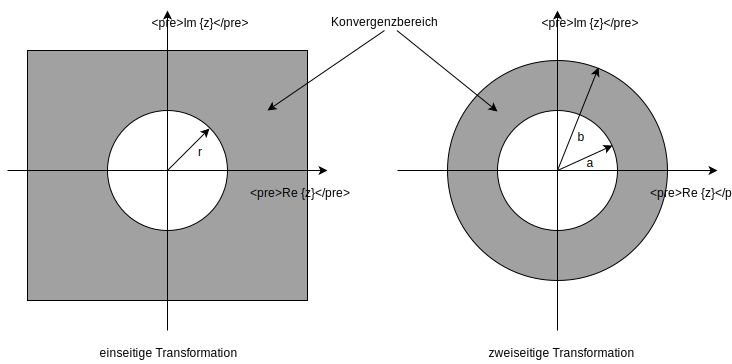
\includegraphics{Konvergenzbereich.svg}
\caption{Konvergenzbereich}
\end{figure}

\begin{itemize}
\tightlist
\item
  Allgemein lässt sich sagen, dass die Z-Transformierte von
  zeitbegrenzten Signalen keine Konvergenzprobleme aufweisst.
\end{itemize}

    \section{Rechenregeln}\label{rechenregeln}

\subsection{Linearität}\label{linearituxe4t}

\begin{itemize}
\item
  Die Z-Transformation ist genau wie die Fourier-Transformation und die
  Laplace-Transformation eine lineare Transformation
\item
  Es seien \(x_1[k]\) und \(x_2[k]\) zwei diskrete Folgen .
\item
  Durch Einsetzen in die Definitionsgleichung erhält man
  \[\mathcal{Z}\{\alpha_1 \cdot x_1[k] + \alpha_2 \cdot x_2[k]\} =  \sum_{k=0}^\infty (\alpha_1 \cdot x_1[k] + \alpha_2 \cdot x_2[k]) \cdot z^{-k}\]
\item
  Die Summe kann aufgeteilt werden in
  \[\sum_{k=0}^\infty \alpha_1 \cdot x_1[k] \cdot z^{-k} + \sum_{k=0}^\infty \alpha_2 \cdot x_2[k] \cdot z^{-k}\]
\item
  Die Konstanten Faktoren \(\alpha_1\) und \(\alpha_2\) können aus der
  Summe gezogen werden
  \[\alpha_1 \sum_{k=0}^\infty \cdot x_1[k] \cdot z^{-k} + \alpha_2 \sum_{k=0}^\infty \cdot x_2[k] \cdot z^{-k}\]
\item
  Die einzelnen Summen können dann durch Gleichung 1.1 ersetzt werden
  \[\alpha_1 \cdot X_1(z) + \alpha_2 \cdot X_2(z)\]
\item
  Damit gilt
  \[\mathcal{Z}\{\alpha_1 \cdot x_1[k] + \alpha_2 \cdot x_2[k]\} = \alpha_1 \cdot X_1(z) + \alpha_2 \cdot X_2(z)\textrm{  (2.1)}\]
\end{itemize}

    \subsection{Zeitinvarianz /
Verschiebungssatz}\label{zeitinvarianz-verschiebungssatz}

\begin{itemize}
\item
  Es sei \(x[k]\) eine kausale und diskrete Folge
\item
  Bei der verschiebung im Zeitbereich ändert sich bei einer zweiseitigen
  Z-Transformation der Konvergenzbereich \(\mathcal{K}\) nicht. Bei
  einer einseitigen Z-Transformation werden Glieder aus dem nicht
  kausalen Bereich eingeschoben, bzw. aus dem kausalen Bereich
  rausgeschoben. .....
\end{itemize}

\subsubsection{Rechtsverschiebung}\label{rechtsverschiebung}

\begin{itemize}
\item
  Durch Einsetzen in die Definitionsgleichung erhält man
  \[\mathcal{Z}\{x[k-k_0]\} = \sum_{k=0}^\infty x[k-k_0] \cdot z^{-k}\]
\item
  Da das Signal Kausal ist, gilt für \(k \lt k_0\) \(x[k-k_0] = 0\).
  Damit lässt sich die untere Summationsgrenze mit \(k=k_0\) ersetzen
  \[\sum_{k=k_0}^\infty x[k-k_0] \cdot z^{-k} = \sum_{k=0}^\infty x[k] \cdot z^{-(k+k_0)}\]
\item
  Damit lässt sich \(z^{-(k+k_0)}\) in eine Konstante und eine variable
  aufspalten \[\sum_{k=0}^\infty x[k] \cdot z^{-k} \cdot z^{-k_0}\]
\item
  Die Konsante kann dann mit den Summenregeln vor die Summe gezogen
  werden \[z^{-k_0} \cdot \sum_{k=0}^\infty x[k] \cdot z^{-k}\]
\item
  Dadurch kann die Summe durch die Gleichung 1.1 ersetzt werden
  \(z^{-k_0} \cdot X(z)\)
\item
  Damit gilt
  \[\mathcal{Z}\{x[k-k_0]\} = z^{-k_0} \cdot X(z)\textrm{  (2.2)}\]
\end{itemize}

\subsubsection{Linksverschiebung}\label{linksverschiebung}

\begin{itemize}
\item
  Die linksverschiebung lässt sich ähnlich wie die Rechtsverschiebung
  herleiten
\item
  Damit gilt
  \[\mathcal{Z}\{x[k+k_0]\} = z^{k_0} \cdot X(z) - z^{k_0} \cdot \sum_{k=0}^{K_0-1}x[k] \cdot z^{-k} = z^{k_0} \cdot (X(z) - \sum_{k=0}^{K_0-1}x[k] \cdot z^{-k})\textrm{  (2.3)}\]
\end{itemize}

    \subsection{Differenz (Ableitung im
Zeitbereich)}\label{differenz-ableitung-im-zeitbereich}

\begin{itemize}
\item
  Die erste Differenz eines Signals ist gegeben mit \(x[k] - x[k-1]\).
\item
  Eingesetzt in die Transformationsgleichung
  \(\mathcal{Z}\{x[k] - x[k-1]\}\) lässt sich die Differenz direkt durch
  den Linearitätssatz und den Verschiebungssatz herleiten.
\item
  Mit dem Linearitätssatz ergibt sich
  \[\mathcal{Z}\{x[k] - x[k-1]\} = \mathcal{Z}\{x[k]\} - \mathcal{Z}\{x[k-1]\}\]
\item
  Mit dem Verschiebungssatz ergibt sich
  \[\mathcal{Z}\{x[k]\} - \mathcal{Z}\{x[k-1]\} = z^0 \cdot X(z) - z^{-1} \cdot X(z) = (1-z^{-1}) \cdot X(z) = \frac{z-1}{z} \cdot X(z)\]
\item
  Damit gilt
  \[\mathcal{Z}\{x[k] - x[k-1]\} = \frac{z-1}{z} \cdot X(z)\textrm{  (2.4)}\]
\item
  Bei der diskreten Ableitung bleibt der Konvergenzbereich
  \(\mathcal{K}\) unverändert.
\end{itemize}

    \subsection{Summation (Integration)}\label{summation-integration}

\begin{itemize}
\item
  Die Summation über einen gewissen Bereich einer Folge \(x[k]\) wird
  beschrieben durch \(x[k] = \sum_{i=0}^k x[i] - \sum_{i=0}^{k-1} x[i]\)
\item
  Eingesetzt in die Transformationsgleichung
  \(\mathcal{Z}\{x[k]\} = \mathcal{Z} \{\sum_{i=0}^k x[i] - \sum_{i=0}^{k-1} x[i]\}\)
  lässt sich die Summation mit dem Differenzsatz 2.4 herleiten
\item
  Mit dem Differenzsatz ergibt sich
  \[X(z) = \mathcal{Z} \{\sum_{i=0}^k x[i] - \sum_{i=0}^{k-1} x[i]\} = \frac{z-1}{z} \cdot \mathcal{Z}\big( \sum_{i=0}^k x[i] \big)\]
\item
  Damit gilt
  \[\mathcal{Z}\big( \sum_{i=0}^k x[i] \big) = \frac{z-1}{z} \cdot X(z)\textrm{  (2.5)}\]
\item
  Bei der diskreten Integration ergibt sich der neue Konvergenzbereich
  aus einer Teilmenge des alten Konvergenzbereichs und demm Bereich
  \({|z| \gt 1}\).
  \[\mathcal{K} \supseteq \mathcal{K}_x \cap {|z| \gt 1}\]
\end{itemize}

    \subsection{Faltung}\label{faltung}

\begin{itemize}
\item
  Die Faltung zweier diskreter Signale ist definiert durch
  \(y = x_1 * x_2 = \sum_{k=-\infty}^\infty x_1[k] \cdot x_2[n-k]\)
\item
  Da die Z-Transformation für Kausale Systeme betrachtet wird gilt
  \(x[k] = 0\) für \(k \lt 0\)
\item
  Damit ergibt sich für die Z-Transformation
  \[\mathcal{Z} \{x_1[k] * x_2[k]\} = \mathcal{Z} \{\sum_{k=0}^\infty x_1[k] \cdot x_2[n-k]\}\]
\item
  Eingesetzt in die Definitionsgleichung 1.1 ergibt sich
  \[\sum_{k=0}^\infty \sum_{i=0}^\infty x_1[i] \cdot x_2[k-i] \cdot z^{-k}\]
\item
  Vertauschung der Summationsreihenfolge
  \[\sum_{i=0}^\infty \sum_{k=0}^\infty x_1[i] \cdot x_2[k-i] \cdot z^{-k}\]
\item
  Damit ist \(x_1[i]\) für die innere Summe eine Konstante, damit gilt
  \[\sum_{i=0}^\infty x_1[i] \cdot \sum_{k=0}^\infty x_2[k-i] \cdot z^{-k}\]
\item
  Durch das Erweitern der inneren Summe mit \(z^{-i} \cdot z^{i} = 1\)
  ergibt sich
  \[\sum_{i=0}^\infty x_1[i] \cdot \sum_{k=0}^\infty x_2[k-i] \cdot z^{-k} \cdot z^{-i} \cdot z^{i}\]
\item
  \(z^{-i} \cdot z^{i}\) sind dabei für die innere Summe konstanten.
  Zieht man \(z^{-i}\) in die äußere Summe ergibt sich
  \[\sum_{i=0}^\infty x_1[i] \cdot z^{-i} \cdot \sum_{k=0}^\infty x_2[k-i] \cdot z^{-k} \cdot z^{i} = \sum_{i=0}^\infty x_1[i] \cdot z^{-i} \cdot \sum_{k=0}^\infty x_2[k-i] \cdot z^{-(k - i)}\]
\item
  Substituiert man dann mit \(k-i = n\) ergibt sich
  \[\sum_{i=0}^\infty x_1[i] \cdot z^{-i} \cdot \sum_{n=0}^\infty x_2[n] \cdot z^{-n} = X_1(z) \cdot X_2(z)\]
\item
  Damit gilt
  \[\mathcal{Z} \{x_1[k] * x_2[k]\} = X_1(z) \cdot X_2(z)\textrm{  (2.6)}\]
\item
  Bei der Faltung ergibt sich der neue Konvergenzbereich aus der
  Schnittmenge der beiden einzelnen Konvergenzbereiche
  \(\mathcal{K} = \mathcal{K}_x \cap \mathcal{K}_y\)
\end{itemize}

    \subsubsection{Beispiel}\label{beispiel}

\begin{itemize}
\item
  gegeben seien zwei Signale \(x_1[k] = \sigma[k]\) und
  \(x_2[k] = h[k]\).
\item
  Die Faltung der Signale ergibt die Sprungantwort des Systems
\item
  Faltet man die Signale im Zeitbereich resultiert dies in einer Summe
  \(a[k] = x_1[k] * x_2[k] = \sum_{i=-\infty}^{\infty} x_1[i] \cdot x_2[k-i]\)
\item
  Transformiert man die Signale aber zuerst in den Zeitbereich
  resultiert die Faltung in einer Multiplikation (siehe 2.6).
\item
  \(A(z) = \mathcal{Z} \{x_1[k] * x_2[k]\} = X_1(z) \cdot X_2(z)\)
\item
  \(A(z)\) muss noch für die endgültige Lösung Rücktransformiert werden.
\item
  Mit dieser Anwendung wird auch die Reihenschaltung von Systemen
  vereinfacht
\end{itemize}

    \subsection{weitere Regeln}\label{weitere-regeln}

\begin{itemize}
\item
  Dämpfungssatz:
  \[a^{-k} \cdot x[k] \circ \!\!-\!\!\bullet X(a \cdot z)\] Der
  Konvergenzradius \(r\) ändert sich um Faktor \(|a|\), womit sich der
  Konvergenzbereich \(\mathcal{K}\) vergrößert.
\item
  Ableitung der Bildfunktion:
  \[k \cdot x[k] \circ \!\!-\!\!\bullet -z \frac{dF(z)}{dz}\] Der
  Konvergenzbereich \(\mathcal{K}\) bleibt unverändert.
\item
  Zeitinversion (nur in der Zweiseitigen Z-Transformation):
  \[x[-k] \circ \!\!-\!\!\bullet X(\frac{1}{z})\] Der Konvergenzbereich
  wird invertiert \(\mathcal{K} = \frac{1}.{\mathcal{K_x}}\)
\item
  Konjugiert komplexe Zeitfolge:
  \[x^{*}[k] \circ \!\!-\!\!\bullet X^{*}(z^{*})\] Der Konvergenzradius
  \(\mathcal{K}\) bleibt unverändert.
\item
  Multiplikationssatz:
  \[w_k \circ \!\!-\!\!\bullet \sum_{k=0}^K u_{K-k} \cdot v_k = \sum_{k=0}^K u_{k} \cdot v_{k-n}\]
\item
  1.Grenzwertsatz:
  \[x[k] = \lim_{z\to\infty} z^k \cdot (X(z) - \sum_{k=0}^{K-1} z^{-k} \cdot x[k]) \textrm{ und } x[k] = \lim_{z\to\infty} X(z)\]
\item
  2.Grenzwertsatz:
  \[\lim_{k\to\infty} x[k] = \lim_{z\to 1} (z-1)\cdot X(z)\]
\item
  Upsampling (Einfügen von nullen):
  \[x[\frac{k}{N}], \frac{k}{N} \in\mathrm{Z} \circ \!\!-\!\!\bullet X(Z^N)\]
  Der neue Konvergenzbereich ist Teilmenge der n-ten Wurzel des alten
  Konvergenzbereiches,
  \(\mathcal{K} \supseteq \sqrt[N]{\mathcal{K}_x}\).
\item
  Stabilität: Für alle Polstellen gilt \(|z| < 1\) -\textgreater{}
  asymptotische Stabilität
\end{itemize}

    \subsubsection{Beispiel}\label{beispiel}

\begin{itemize}
\item
  Gegeben sei die Übertragungsfunktion aus dem ersten Beispiel
  \(H(z) = \frac{z^2 + 2z + 1}{z^2}\)
\item
  Ist das System \(H(z)\) stabil?
\item
  Ob das system Stabil ist kann einfach über den Pol-/ und
  Nullstellenplan bestimmt werden
\item
  Für die Nullstellen gilt: \(z^2 + 2z + 1 = 0\)

  \begin{itemize}
  \tightlist
  \item
    \(z_{0,1} = z_{0,2} = -1\)
  \end{itemize}
\item
  Für die Polstellen gilt \(z^2 = 0\)

  \begin{itemize}
  \tightlist
  \item
    \(z_{\infty,1} = z_{\infty,2} = 0\)
  \end{itemize}
\item
  Da für alle Polstellen \(|z_{\infty,i}| < 1\) erfüllt ist, ist
  \(H(z)\) stabil.
\end{itemize}

    \subsection{Korespondenztabelle für die
Z-Transformation}\label{korespondenztabelle-fuxfcr-die-z-transformation}

\begin{longtable}[]{@{}lll@{}}
\toprule
\begin{minipage}[b]{0.05\columnwidth}\raggedright\strut
Nr\strut
\end{minipage} & \begin{minipage}[b]{0.28\columnwidth}\raggedright\strut
Signal \(x[k]\)\strut
\end{minipage} & \begin{minipage}[b]{0.58\columnwidth}\raggedright\strut
Z-Transformierte \(X(z)\)\strut
\end{minipage}\tabularnewline
\midrule
\endhead
\begin{minipage}[t]{0.05\columnwidth}\raggedright\strut
1\strut
\end{minipage} & \begin{minipage}[t]{0.28\columnwidth}\raggedright\strut
\(\delta[k]\)\strut
\end{minipage} & \begin{minipage}[t]{0.58\columnwidth}\raggedright\strut
\(1\)\strut
\end{minipage}\tabularnewline
\begin{minipage}[t]{0.05\columnwidth}\raggedright\strut
2\strut
\end{minipage} & \begin{minipage}[t]{0.28\columnwidth}\raggedright\strut
\(\sigma[k]\)\strut
\end{minipage} & \begin{minipage}[t]{0.58\columnwidth}\raggedright\strut
\(\frac{z}{z-1}\)\strut
\end{minipage}\tabularnewline
\begin{minipage}[t]{0.05\columnwidth}\raggedright\strut
3\strut
\end{minipage} & \begin{minipage}[t]{0.28\columnwidth}\raggedright\strut
\(k \cdot \sigma[k]\)\strut
\end{minipage} & \begin{minipage}[t]{0.58\columnwidth}\raggedright\strut
\(\frac{z}{(z-1)^2}\)\strut
\end{minipage}\tabularnewline
\begin{minipage}[t]{0.05\columnwidth}\raggedright\strut
4\strut
\end{minipage} & \begin{minipage}[t]{0.28\columnwidth}\raggedright\strut
\(k^2 \cdot \sigma[k]\)\strut
\end{minipage} & \begin{minipage}[t]{0.58\columnwidth}\raggedright\strut
\(\frac{z\cdot(z+1)}{(z-1)^{-3}}\)\strut
\end{minipage}\tabularnewline
\begin{minipage}[t]{0.05\columnwidth}\raggedright\strut
5\strut
\end{minipage} & \begin{minipage}[t]{0.28\columnwidth}\raggedright\strut
\(\lambda^k \cdot \sigma[k]\)\strut
\end{minipage} & \begin{minipage}[t]{0.58\columnwidth}\raggedright\strut
\(\frac{z}{z-\lambda}\)\strut
\end{minipage}\tabularnewline
\begin{minipage}[t]{0.05\columnwidth}\raggedright\strut
6\strut
\end{minipage} & \begin{minipage}[t]{0.28\columnwidth}\raggedright\strut
\(k\cdot\lambda^k\cdot\sigma[k]\)\strut
\end{minipage} & \begin{minipage}[t]{0.58\columnwidth}\raggedright\strut
\(\frac{z\cdot\lambda}{(z-\lambda)^2}\)\strut
\end{minipage}\tabularnewline
\begin{minipage}[t]{0.05\columnwidth}\raggedright\strut
7\strut
\end{minipage} & \begin{minipage}[t]{0.28\columnwidth}\raggedright\strut
\(k^2\cdot\lambda^k\cdot\sigma[k]\)\strut
\end{minipage} & \begin{minipage}[t]{0.58\columnwidth}\raggedright\strut
\(\frac{z\cdot\lambda\cdot(z+\lambda)}{(z-\lambda)^3}\)\strut
\end{minipage}\tabularnewline
\begin{minipage}[t]{0.05\columnwidth}\raggedright\strut
8\strut
\end{minipage} & \begin{minipage}[t]{0.28\columnwidth}\raggedright\strut
\(k^3\cdot\lambda^k\cdot\sigma[k]\)\strut
\end{minipage} & \begin{minipage}[t]{0.58\columnwidth}\raggedright\strut
\(\frac{z\cdot\lambda\cdot(z^2+4\cdot\lambda\cdot z+ \lambda^2)}{(z-\lambda)^4}\)\strut
\end{minipage}\tabularnewline
\begin{minipage}[t]{0.05\columnwidth}\raggedright\strut
9\strut
\end{minipage} & \begin{minipage}[t]{0.28\columnwidth}\raggedright\strut
\(\sin (k\cdot\Omega_0)\cdot\sigma[k]\)\strut
\end{minipage} & \begin{minipage}[t]{0.58\columnwidth}\raggedright\strut
\(\frac{z\cdot\sin(\Omega_0)}{z^2-2\cdot z\cdot\cos(\Omega_0)+1}\)\strut
\end{minipage}\tabularnewline
\begin{minipage}[t]{0.05\columnwidth}\raggedright\strut
10\strut
\end{minipage} & \begin{minipage}[t]{0.28\columnwidth}\raggedright\strut
\(\cos (k\cdot\Omega_0)\cdot\sigma[k]\)\strut
\end{minipage} & \begin{minipage}[t]{0.58\columnwidth}\raggedright\strut
\(\frac{z\cdot\cos(\Omega_0)}{z^2-2\cdot z\cdot\cos(\Omega_0)+1}\)\strut
\end{minipage}\tabularnewline
\bottomrule
\end{longtable}

    \begin{itemize}
\tightlist
\item
  Der Konvergenzbereich genügt der bedingung \(|z| \geq 1\) bzw.
  \(|z| \geq \lambda\) mit \(z, \lambda\in \mathcal{C}\)
\end{itemize}

    \section{Rücktransformation / inversen
Z-Transformation}\label{ruxfccktransformation-inversen-z-transformation}

\begin{itemize}
\item
  Die inverse Z-Transformation ist gegebeben mit
  \(x[k] = \mathcal{Z}^{-1} \cdot X(z)\)
\item
  Die Integraldarstellung hat die Form
  \[x[k] = \big( \frac{1}{2\pi j} \big) \cdot \oint X(z) \cdot z^{k-1}\,dz\]
\item
  Meistens entsehen bei der Z-Transformation gebrochen Rationale
  Funktionen wie im 1. Beispiel
\item
  Deren Rücktransformation kann am einfachsten über die
  Partialbruchzerlegung durchgeführt werden. Diese Methode zerlegt eine
  komplizierte algebraische Funktion in elementare Terme. Diese
  elementaren Terme können dann einfach transformiert werden. Eine
  weitere Möglichkeit is es diese durch den Residuensatz
  durchzuführen.Eine ditte Möglichkeit der Rücktransformation ist das
  komplexe Umkehrintegral.
\item
  Die Rücktransformation wird nur für den praktisch relvanten Fall der
  kausalen Signale betrachtet.
\end{itemize}

    \subsection{inverse Z-Transformation über
Partialbruchzerlegung}\label{inverse-z-transformation-uxfcber-partialbruchzerlegung}

\begin{itemize}
\item
  gegeben sind zwei Ganz Rationale Funktinen \(A(z)\) und \(B(z)\).
\item
  Gesucht ist X(z)\$ \bullet !!-!!\circ x{[}k{]}\$
  \[X(z) = \frac{B(z)}{A(z)} = \frac {\sum_{i=0}^M b_i \cdot z^{i}} {\sum_{i=0}^N a_i \cdot z^{i}} = \frac{b_0 + b_1 \cdot z^1 + ... + b_M \cdot z^N}{a_0 + a_1 \cdot z^1 + ... + a_N \cdot z^N}\]
\item
  Für die Partialbruchzerlegung muss der Grad des Nennerpolynoms größer
  als der Grad des Zählerpolynoms sein.
\item
  Da es Sich bei \(A(z)\) und \(B(z)\) jeweils um Kausale Signale
  handelt ist der Grad von \(A(z)\) maximal so groß wie der Grad
  \(B(z)\).
\item
  Tritt der Fall ein, das \(M = N\) muss vor der Partialbruchzerlegung
  eine Polynomdivision durchgeführt werden.
\item
  Als Ergebnis dieser Polynomdivision ist ein konstanter Summand
  \(X_0 = \frac{b_M}{a_N}\).
\item
  Ist \(X(z)\) dann eine echt gebrochen Rationale Funktion werden die
  Pole bestimmt. Diese entsprechen den Nullstellen der Funtion \(A(z)\).
\item
  Je nach Vielfachheit der Polstelle werden dann verschiedene Ansätze
  für den Koeffizientenvergleich gewählt
\end{itemize}

    \subsubsection{\texorpdfstring{einfacher Pol an
\(z \neq 0\)}{einfacher Pol an z \textbackslash{}neq 0}}\label{einfacher-pol-an-z-neq-0}

\[ X(z) = \frac{B(z)}{A(z)} = \frac{A}{z-\alpha_1} + \frac{B}{z-\alpha_2} + ... + \frac{Q}{z-\alpha_n}\]

\begin{itemize}
\tightlist
\item
  Multiplikation mit \(A(z)\) um die Gleichung auf den Haupnenner
  \(A(z)\) zu bringen.
\end{itemize}

\[ B(z) = \frac{A\cdot A(z)}{z-\alpha_1} + \frac{B\cdot A(z)}{z-\alpha_2} + ... + \frac{Q\cdot A(z)}{z-\alpha_n}\]

\begin{itemize}
\item
  Mit diesem Schritt ergeben sich durch den Koeffizientenvergleich n
  gleichungen der Form \(C_i * C(z) = \frac{a_i\cdot A(z)}{z-\alpha_i}\)
\item
  Aus diesen Gleichungen kann ein LGS Aufgestellt werden um alle \(a_n\)
  zu berrechnen.
\item
  Anschließend hat jeder der partialbrüche die Form
  \(X_i(z) = \frac{C_i}{z-\alpha_i}\) mit \(C_i = \{A, B, ..., Q\}\)
\item
  Diese Partialbrücke können über die Korrespondenztabelle in eine um 1
  nach rechts verschobene kausale Exponentialfolge überführt werden.
\end{itemize}

\[X_i[k] = \mathcal{Z}\big\{\frac{C_i}{z-\alpha_i}\big\} = C_i \cdot \alpha_i^{k-1} \cdot \sigma[k-1]\]

\begin{itemize}
\tightlist
\item
  Summiert man alle \(X_n[k]\) auf ergibt sich die Folge im Zeitbereich
  \[x[k] = \sum_{i=1}^N C_i \cdot \alpha_i^{k-1} \cdot \sigma[k-1]\]
\end{itemize}

    \subsubsection{\texorpdfstring{mehrfacher Pol an
\(z \neq 0\)}{mehrfacher Pol an z \textbackslash{}neq 0}}\label{mehrfacher-pol-an-z-neq-0}

\begin{itemize}
\item
  \[G(z) = \frac{Y(z)}{X(z)} = \frac{a_1}{z-x_{is_0}} + \frac{a_2}{z-x_{is_0}} + ... + \frac{a_q}{z-x_{is_0}}\]
\item
  \[g[k] = \sum_{n=1}^P a_n\cdot X(z) \cdot \binom{k-1}{n-1} \cdot x_{ps_n}^{k-n} \cdot \sigma[k-n]\]
\end{itemize}

    \subsubsection{\texorpdfstring{Sonderfall mehrfacher Pol an
\(z = 0\)}{Sonderfall mehrfacher Pol an z = 0}}\label{sonderfall-mehrfacher-pol-an-z-0}

\begin{itemize}
\item
\end{itemize}

    \subsubsection{Beispiel}\label{beispiel}

\begin{itemize}
\tightlist
\item
  Gegeben ist die Gleichung
  \(X(z) = \frac{z}{z^2 + 3 \cdot z + 2} = \frac{z}{(z+1) \cdot (z+2)}\)
\item
  Die zugehörigen Polstellen sind \$\alpha\_0 = -1 ;\alpha\_1 = -2 \$
\item
  Für den Koeffizientenvergleich ergibts sich wegen der einfachen
  Nullstellen \(z \neq 0\)
  \[X(z) = \frac{z}{(z+1) \cdot (z+2)} = \frac{A}{z+1} + \frac{B}{z+2}\]
\item
  Durch multiplikation mit \((z+1) \cdot (z+2)\) folgt
  \[ z = A \cdot (z+2) + B \cdot (z+1)\]
\item
  Mit dem Koeffizientenvergleich und dem Einsetzen der Nullstellen
  ergibt sich für die Konstanten \(A = -1\) und \(B = 2\).
\item
  Damit ergeben sich die Partialbrüche
  \[ X_1(z) = \frac{-1}{z+1} \textrm{  und  } X_2(z) = \frac{2}{z+2}\]
  \[ X(z) = \frac{-1}{z+1} + \frac{2}{z+2}\]
\item
  Transformiert man dann die Pratialbrücke über die Korrespondenztabelle
  ergibt sich
  \[x[k] = -1 \cdot (-1)^{k-1} \cdot \sigma[k-1] + 2 \cdot (-2)^{k-1} \cdot \sigma[k-1]\]
\end{itemize}

    \paragraph{Daarstellung der
Pol-/Nullstellen}\label{daarstellung-der-pol-nullstellen}

\begin{itemize}
\tightlist
\item
  Polstellen werden im Koordinatensystem als kreuze markiert,
  Nullstellen als Kreise. 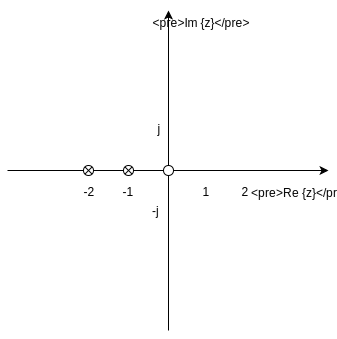
\includegraphics{Pol_Null_S.svg}
\end{itemize}

    \section{Bezug zur Laplace-Transformation und
Fourier-Transformation}\label{bezug-zur-laplace-transformation-und-fourier-transformation}

\begin{itemize}
\item
  Da es sich bei der Fourier-Transformation lediglich um einen
  Spezialfall der Laplace-Transformation handelt, wird der zusammenhang
  mit der Laplace-Transformation beschrieben
\item
  Die Laplace-Transformation ist eine Transformation für
  zeitkontinuierliche Signale. Sie transformiert das System aus dem
  Zeitbereich in den Frequenzbereich. Im Frequenzbereich kann das
  mathematische Problem dann einfacher gelößt werden. Anschließend kann
  durch die Rücktransformation, auch inverse Laplace-Transformation
  genannt, die Lösung dann zurück in den Zeitbereich transformiert
  werden.
\item
  Schon bei der Herleitung der Definitionsgleichung 1.5 der
  Z-Transformation wurde der Ansatz über die Laplace-Transformation
  gewählt. Dies liegt an dem Zusammenhang der beiden Transformationen.
  Die Z-Transformation ist das Äquivalent zur Laplace-Transformation für
  den Zeitdiskreten Fall.
\item
  Mit der Substitution \(t = e^{T_A \cdot s}\) aus der Herleitung der
  Definitionsgleichung wird die komplexe s-Ebene in die komplexe z-Ebene
  abgebildet s-Ebene z-Ebene
\end{itemize}

\begin{longtable}[]{@{}ll@{}}
\toprule
s-Ebene & z-Ebene\tabularnewline
\midrule
\endhead
imaginäre-Achse & Einheitskreis\tabularnewline
linke komplexe Ebene & Inneres des Einheitskreises\tabularnewline
rechte komplexe Ebene & Äuseres des Einheitskreises\tabularnewline
Ursprung \(s = 0\) & \(z = 1\)\tabularnewline
\bottomrule
\end{longtable}

    \subsection{Lösung einer
Differenzengleichung}\label{luxf6sung-einer-differenzengleichung}

\begin{itemize}
\tightlist
\item
  Gegeben ist eine Differenzengleichung der Form
  \(\sum_{i=0}^V a_i \cdot y[k-i] = \sum_{i=0}^U b_i \cdot x[k-i]\)
  \#\#\# ohne Anfangsbedingungen
\item
  Diese Gleichung kann mit der Rechtsverschiebung (2.2) in eine
  Z-Transformierte Gleichung überführt werden.
  \[\sum_{i=0}^V a_i \cdot Y(z) \cdot z^{-i} = \sum_{i=0}^U b_i \cdot X(z) \cdot z^{-i}\]
\item
  Die Z-Transformierten \(X(z)\) und \(Y(z)\) können aus den Summen
  Ausgeklamert werden.
  \[Y(z) \cdot \sum_{i=0}^V a_i \cdot z^{-i} = X(z) \cdot \sum_{i=0}^U b_i \cdot z^{-i}\]
\item
  Anschließend kann die Gleichung nach der Z-Transformierten des
  Ausgangssignals aufgelöst werden.
  \[Y(z) = X(z) \cdot \frac{\sum_{i=0}^U b_i \cdot z^{-i}}{\sum_{i=0}^V a_i \cdot z^{-i}}\]
\item
  Die Ausgangsgleichung kann dann entweder über die inverse
  Z-Transformation mittels Residuensatz oder Partialbruchzerlegung in
  den Zeitbereich zurücktransformiert werden.
\end{itemize}

    \subsubsection{mit Anfangsbedingungen}\label{mit-anfangsbedingungen}

\begin{itemize}
\tightlist
\item
  Existieren Anfangsbedingungen muss das System von diesen Anfangswerten
  aus betrachtet werden. Mit der gegebenen Zeitinvarianz des Systems
  kann dies durch eine einfache verschiebung nach links durchgeführt
  werden. \[ 
  \sum_{i = 0}^V a_{V-i} \cdot y[k-i+V]
  =
  \sum_{i = 0}^U b_{U-i} \cdot x[k-i+U]
  \]
\end{itemize}

    \begin{itemize}
\tightlist
\item
  In impliziter daarstellung folgt \[
  y[k] 
  = \frac{1}{a_V} 
  - \sum_{i = 1}^V a_{V-i} \cdot y[k-i+V]
  + \sum_{i = 0}^U b_{U-i} \cdot x[k-i+U]
  \]
\end{itemize}

    \begin{itemize}
\tightlist
\item
  Zuerst wird die Homogene Lösung behandelt \[
  \sum_{i = 0}^V a_{V-i} \cdot y[k-i+V] = 0
  \]
\end{itemize}

    \begin{itemize}
\tightlist
\item
  Transformation in den Z-Bereich über die Verschiebungsregel. \[
  a_0 \cdot Y(z) + \sum_{i = 1}^{N} a_i \big( z^{i} \cdot Y(z) 
  - \sum_{j = 0}^{i - 1} y[j] \cdot z^{i-j} \big) 
  = 0
  \]
\end{itemize}

    \[
    a_0 \cdot Y(z) 
    + \sum_{i = 1}^{N} a_i \big( z^{i} \cdot Y(z) 
    - \sum_{j = 0}^{i - 1} y[j] \cdot z^{i-j} \big) 
    = 0
\]

    \begin{itemize}
\tightlist
\item
  Anschließend kann die Gleichung mit der Linksverschiebung (2.3) in
  eine Z-Transformierte Gleichung überführt werden.
  \[\sum_{i=0}^V a_i \cdot \big(Y(z) \cdot z^{V-i} - z^{V-i} \cdot \sum_{k = 0}^{V-i-1} y[k] \cdot z^{-k}\big) = \sum_{i=0}^U b_i \cdot \big(X(z) \cdot z^{U-i} - z^{U-i} \cdot \sum_{k = 0}^{U-i-1} x[k] \cdot z^{-k}\big)\]
\end{itemize}

    \subsubsection{Beispiel}\label{beispiel}

\begin{itemize}
\tightlist
\item
  Anhand des Autonomen Systems der fibonacci Folge aus der Vorlesung mit
  den Anfangsbedingungen \(y[0] = y[1] = 1\) \[y[k] = y[k-1] + y[k-2] \]
\end{itemize}

    \[ y[k] - y[k-1] - y[k-2] = 0\]

    \begin{itemize}
\tightlist
\item
  Verschiebung um \(2\) nach links \[ y[k+2] - y[k+1] - y[k] = 0\]
\end{itemize}

    \begin{itemize}
\tightlist
\item
  Transformation in den Z-Bereich über die Linksverschiebung. Alle
  \(a_i = 0\), \(V = 2\). \$\$ Y(z) \cdot z\^{}2 - z\^{}2
  \cdot \big(\sum\_\{k=0\}\^{}\{1\} y{[}k{]} \cdot z\^{}\{-k\}\big)
\item
  (Y(z) \cdot z - z \cdot \big(\sum\_\{k=0\}\^{}\{0\} y{[}k{]}
  \cdot z\^{}\{-k\}\big))
\item
  Y(z) = 0 \$\$
\end{itemize}

    \[
    z^2 Y(z) - z^2 y[0] - z^1 y[1] 
    - (zY(z) - zy[0]) - Y(z)
    = 0
\]

    \[
    z^2 Y(z) - z^2 - z - zY(z) + z - Y(z) = 0
\]

    \[
    Y(z) \cdot (z^2 - z - 1) -z^2 = 0
\]'

    \begin{itemize}
\tightlist
\item
  Bringt man \(Y(z)\) auf die linke Seite ergibt sich \[
  Y(z) = \frac{z^2}{z^2 - z - 1}
  \]
\end{itemize}

    \begin{itemize}
\tightlist
\item
  Diese Gleichung kann mittels Partialbruchzerlegung in den Zeitbereich
  zurücktransformiert werden. Dafür muss zuerst eine Polynomdivision
  durchgeführt werden um eine echt gebrochen Rationale Funktion zu
  erhalten. \[
  \frac {z^2}{z^2 - z - 1} =  1 + \frac{z+1}{z^2 - z - 1}  
  \]
\end{itemize}

    \begin{itemize}
\tightlist
\item
  Damit ist die Konstante \(Y_0\) = 1 bzw \(y[0] = \delta[1]\) und die
  echt gebrochen rationale Funktion \(\frac{z + 1}{z^2 - z - 1}\)
\item
  Die Pole der Funktion sind \(z_{-\infty,0} = \frac{1+\sqrt{5}}{2}\)
  und \(z_{-\infty,1} = \frac{1-\sqrt{5}}{2}\)
\end{itemize}

    \begin{itemize}
\tightlist
\item
  Führt man eine Partialbruchzerlegung durch und transformiert man diese
  mit der Korrespondenztabelle in den Zeitbereich zurück erhält man \[
  y[k] 
  = \frac{1}{\sqrt{5}} \cdot 
      \bigg( 
          \big( \frac{1+\sqrt{5}}{2} \big)^k 
          -
          \big( \frac{1-\sqrt{5}}{2} \big)^k             
      \bigg)        
  \]
\end{itemize}

    \begin{Verbatim}[commandchars=\\\{\}]
{\color{incolor}In [{\color{incolor}16}]:} \PY{o}{\PYZpc{}}\PY{k}{matplotlib} inline
         
         \PY{k+kn}{import} \PY{n+nn}{matplotlib}
         \PY{k+kn}{import} \PY{n+nn}{numpy} \PY{k}{as} \PY{n+nn}{np}
         \PY{k+kn}{import} \PY{n+nn}{matplotlib}\PY{n+nn}{.}\PY{n+nn}{pyplot} \PY{k}{as} \PY{n+nn}{plt}
         \PY{k+kn}{import} \PY{n+nn}{math}
         
         \PY{n}{amount} \PY{o}{=} \PY{l+m+mi}{10}
         \PY{n}{k} \PY{o}{=} \PY{p}{[}\PY{p}{]}
         \PY{k}{for} \PY{n}{i} \PY{o+ow}{in} \PY{n+nb}{range}\PY{p}{(}\PY{n}{amount}\PY{p}{)}\PY{p}{:}
             \PY{n}{k}\PY{o}{.}\PY{n}{append}\PY{p}{(}\PY{n}{i}\PY{p}{)}
         \PY{n}{y} \PY{o}{=} \PY{p}{[}\PY{p}{]}
         \PY{k}{for} \PY{n}{val} \PY{o+ow}{in} \PY{n}{k}\PY{p}{:}
             \PY{n}{first} \PY{o}{=} \PY{n}{math}\PY{o}{.}\PY{n}{pow}\PY{p}{(}\PY{p}{(}\PY{l+m+mi}{1}\PY{o}{+}\PY{n}{math}\PY{o}{.}\PY{n}{sqrt}\PY{p}{(}\PY{l+m+mi}{5}\PY{p}{)}\PY{p}{)}\PY{o}{/}\PY{l+m+mi}{2}\PY{p}{,} \PY{n}{val}\PY{p}{)}
             \PY{n}{second} \PY{o}{=} \PY{n}{math}\PY{o}{.}\PY{n}{pow}\PY{p}{(}\PY{p}{(}\PY{l+m+mi}{1}\PY{o}{\PYZhy{}}\PY{n}{math}\PY{o}{.}\PY{n}{sqrt}\PY{p}{(}\PY{l+m+mi}{5}\PY{p}{)}\PY{p}{)}\PY{o}{/}\PY{l+m+mi}{2}\PY{p}{,} \PY{n}{val}\PY{p}{)}
             \PY{n}{tmp} \PY{o}{=} \PY{p}{(}\PY{p}{(}\PY{l+m+mi}{1}\PY{o}{/}\PY{n}{math}\PY{o}{.}\PY{n}{sqrt}\PY{p}{(}\PY{l+m+mi}{5}\PY{p}{)}\PY{p}{)}\PY{o}{*}\PY{p}{(}\PY{n}{first} \PY{o}{\PYZhy{}} \PY{n}{second}\PY{p}{)}\PY{p}{)}
             \PY{n}{y}\PY{o}{.}\PY{n}{append}\PY{p}{(}\PY{n}{tmp}\PY{p}{)}
         \PY{n}{plt}\PY{o}{.}\PY{n}{stem}\PY{p}{(}\PY{n}{k}\PY{p}{,}\PY{n}{y}\PY{p}{)}
\end{Verbatim}


\begin{Verbatim}[commandchars=\\\{\}]
{\color{outcolor}Out[{\color{outcolor}16}]:} <StemContainer object of 3 artists>
\end{Verbatim}
            
    \begin{center}
    \adjustimage{max size={0.9\linewidth}{0.9\paperheight}}{output_45_1.png}
    \end{center}
    { \hspace*{\fill} \\}
    
    \subsection{Signalflussplan}\label{signalflussplan}

Die Darstellung einer Differenzengleichung im Signalflussplan wurde
schon in der Vorlesung vorgestellt.

    \section{Übertragungsglieder}\label{uxfcbertragungsglieder}

    \section{Beispiel}\label{beispiel}

    \subsection{Zusammenfassung}\label{zusammenfassung}

\begin{itemize}
\tightlist
\item
  Die Z-Transformation ist eines der wichtigsten Hilfsmittel zur Lösung
  von linearen Differenzengleichungen mit konstanten Koeffizienten. Sie
  vereinfacht die Theorie der diskreten LTI-Systeme und das Lösen der
  gegebenen mathematischen Probleme. Aus komplexen Faltungen im
  Zeitbereich zum bestimmen von Übertragungsgleichungen oder
  Systemantworten wird eine einfache Multiplikation im Z-Bereich. Sofern
  eine Z-Transformierte für ein diskretes LTI-System existiert ist es
  mit der einfachste Weg das System mit der Z-Transformation zu
  entschlüsseln.
\end{itemize}


    % Add a bibliography block to the postdoc
    
    
    
    \end{document}
